\chapter{Funkcja logiczna jednego segmentu wskaźnika 7-segmentowego}

\section{Stworzenie funkcji logicznej}

\begin{itemize}
    \item Należało zbudować funkcję logiczną dla jednego z segmentów wskaźnika:
        \begin{figure}[H]
            \centering
            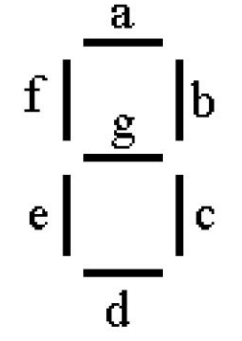
\includegraphics[width=0.3\textwidth]{img/dodatkowe/wskaznik.png}
            \caption{Wskaźnik 7-segmentowy}
            \label{dodatkowe:schemat_wskaznika}
        \end{figure}
    \item Dla segmentu \textbf{c} tablica sygnałów wejściowych (liczb w zapisie binarnym (\textbf{BIN}), oraz ich konwersja na dziesiętne (\textbf{DEC})) oraz wyjściowych (czy segment powinien być zapalony) wygląda w następujący sposób:
        \begin{center}
            \label{dodatkowe:teor_funkcja}
            \begin{tabular}{|c|c|>{\columncolor[gray]{0.8}}c|}
                \hline
                DEC & BIN & Y \\
                \hline
                0 & 000 & \textcolor{red}{1} \\
                \hline
                1 & 001 & \textcolor{red}{1} \\
                \hline
                2 & 010 & 0 \\
                \hline
                3 & 011 & \textcolor{red}{1} \\
                \hline
                4 & 100 & \textcolor{red}{1} \\
                \hline
                5 & 101 & \textcolor{red}{1} \\
                \hline
                6 & 110 & \textcolor{red}{1} \\
                \hline
                7 & 111 & \textcolor{red}{1} \\
                \hline
            \end{tabular}
        \end{center}
\pagebreak

    \item Mapa Karnaugh'a wykorzystana na laboratoriach do minimalizacja funkcji: \\
    \begin{center}
        \begin{karnaugh-map}[4][2][1][$BC$][$A$]
            \maxterms{2}
            \minterms{0,1,3,4,5,6,7}
            \implicant{0}{4}
            \implicant{1}{5}
            \implicant{7}{6}
        \end{karnaugh-map}
    \end{center}
        
    \item Otrzymana funkcja na laboratorium:
        \begin{equation}
            F = \overline{B}\overline{C} + \overline{B}C + AB + \overline{A}BC
        \end{equation}
        Po uproszczeniu:
        \begin{equation}
            \label{dodatkowe:lab_equation}
            F = \overline{B}(\overline{C}+C)+AB+\overline{A}BC = \overline{B}+B(A+\overline{A}C) = \overline{\textbf{B}}\textbf{+B(A+C)}
        \end{equation}
        Równanie wyżej można dodatkowo uprościć (co nie zostało wykonane na laboratoriach) do postaci:
        \begin{equation}
            \label{dodatkowe:further_simplified}
            F = \overline{\textbf{B}}\textbf{+A+C}
        \end{equation}
\end{itemize}

\section{Budowa za pomocą bramek}

\begin{itemize}
    \item Korzystając z wyprowadzonego na laboratoriach równania (\ref{dodatkowe:lab_equation}) zaprojektowano 8-bramkowy układ (zamiast bramki not został zastosowany zanegowany sygnał z impulsatora ($\overline{\textbf{Q}}$):
        \begin{figure}[H]
            \centering
            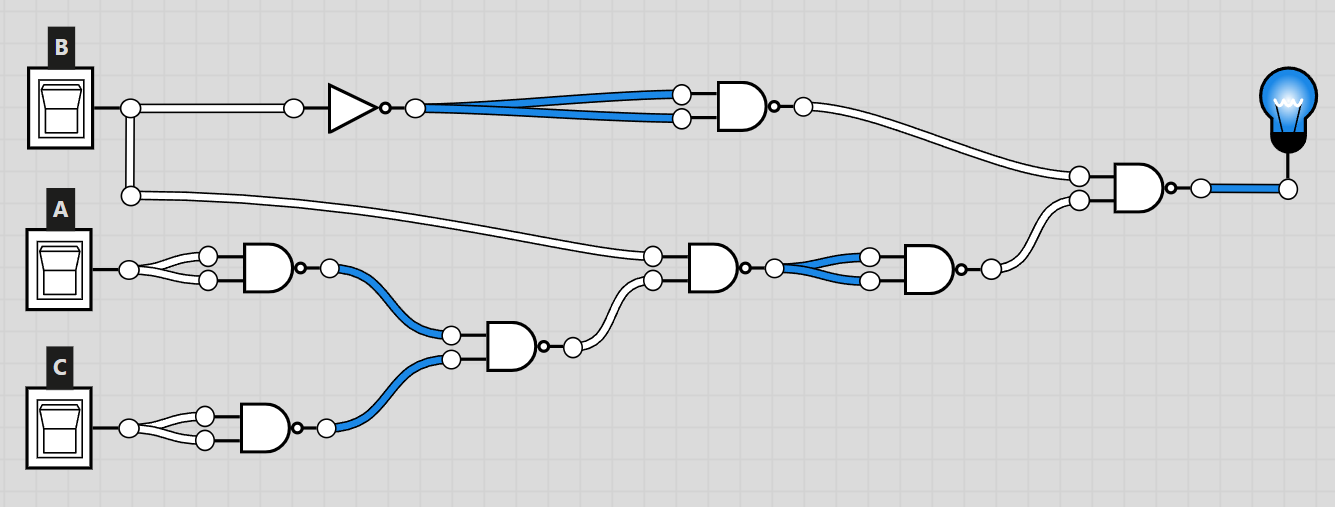
\includegraphics[width=0.8\textwidth]{img/dodatkowe/schemat_lab_w_not.png}
            \caption{}
            \label{dodatkowe:schemat_lab}
        \end{figure}

\pagebreak

    \item Zbudowany układ:
        \begin{figure}[H]
            \centering
            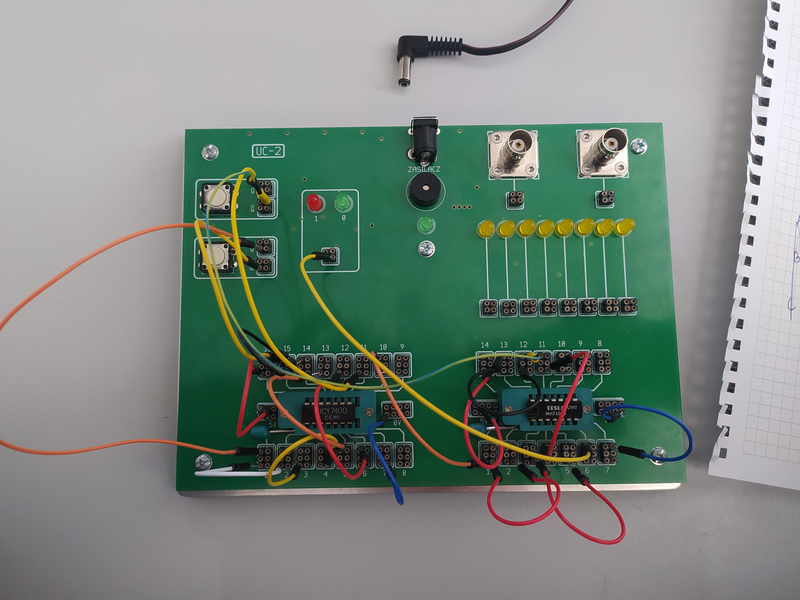
\includegraphics[width=\textwidth]{img/4_5/1652306732304_scaled.png}
            \label{dodatkowe:zbudowany_lab}
        \end{figure}
    \item Niestety, zaprojektowany na laboratoriach układ \textbf{nie realizował} wyprowadzonej funkcji (\ref{dodatkowe:lab_equation}).
    \item Tabela układu (\autoref{dodatkowe:schemat_lab}):
        \begin{center}
            \begin{tabular}{|c|c|c|>{\columncolor[gray]{0.8}}c|}
                \hline
                A & B & C & Y \\
                \hline
                0 & 0 & 0 & 1 \\
                \hline
                0 & 0 & 1 & 1 \\
                \hline
                0 & 1 & 0 & 1 \\
                \hline
                0 & 1 & 1 & 0 \\
                \hline
                1 & 0 & 0 & 1 \\
                \hline
                1 & 0 & 1 & 1 \\
                \hline
                1 & 1 & 0 & 0 \\
                \hline
                1 & 1 & 1 & 0 \\
                \hline
            \end{tabular}
        \end{center}
        \textbf{Nie zgadza się} z przewidywaną tabelą (\ref{dodatkowe:teor_funkcja})
\end{itemize}

\pagebreak

\section{Poprawne rozwiązanie}

\begin{itemize}
    \item Korzystając z najbardziej uproszczonej wersji funkcji logicznej (\ref{dodatkowe:further_simplified}) należałoby stworzyć następujący układ:
        \begin{figure}[H]
            \centering
            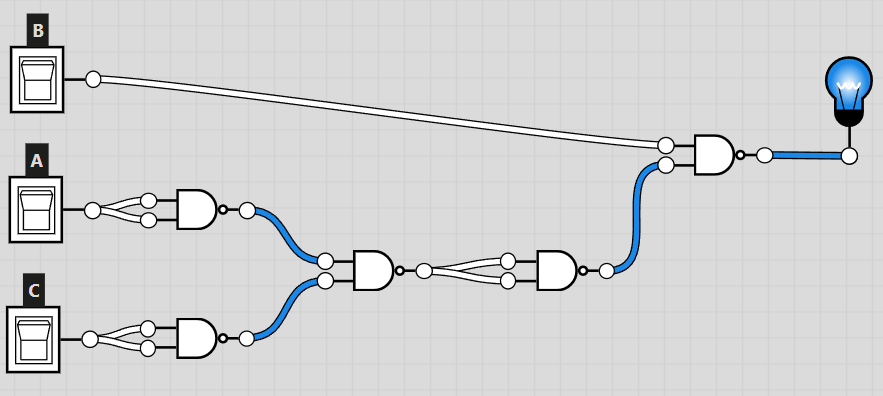
\includegraphics[width=\textwidth]{img/dodatkowe/schemat_poprawny.png}
            \caption{Poprawny układ funkcji \ref{dodatkowe:further_simplified}}
            \label{dodatkowe:poprawny_uklad}
        \end{figure}
    \item Tabela układu powyżej:
        \begin{center}
            \begin{tabular}{|c|c|c|>{\columncolor[gray]{0.8}}c|}
                \hline
                A & B & C & Y \\
                \hline
                0 & 0 & 0 & 1 \\
                \hline
                0 & 0 & 1 & 1 \\
                \hline
                0 & 1 & 0 & 0 \\
                \hline
                0 & 1 & 1 & 1 \\
                \hline
                1 & 0 & 0 & 1 \\
                \hline
                1 & 0 & 1 & 1 \\
                \hline
                1 & 1 & 0 & 1 \\
                \hline
                1 & 1 & 1 & 1 \\
                \hline
            \end{tabular}
        \end{center}
        \textbf{Zgadza się} ona z teoretyczną tabelą wejść i wyjść.
\end{itemize}